%%%%%%%%%%%%%%%%%%%%%%%%%%%%%%%%%%%%%%%%%%%%%%%%%%%%%%%%%%%%%%%%%%%%%%%%%%%

\documentclass{standalone}

\usepackage{amsmath}
\usepackage{mathptmx}
\usepackage{tikz}
\usetikzlibrary{external}
\tikzexternalize{difference-two-squares}

%% IEEE uses Times Roman font, so we'll default to Times.
%% These three commands make up the entire times.sty package.
\renewcommand{\rmdefault}{ptm}
\renewcommand{\ttdefault}{pcr}
\normalfont\selectfont

%%%%%%%%%%%%%%%%%%%%%%%%%%%%%%%%%%%%%%%%%%%%%%%%%%%%%%%%%%%%%%%%%%%%%%%%%%%
%% Difference of two squares.
%%%%%%%%%%%%%%%%%%%%%%%%%%%%%%%%%%%%%%%%%%%%%%%%%%%%%%%%%%%%%%%%%%%%%%%%%%%

\begin{document}

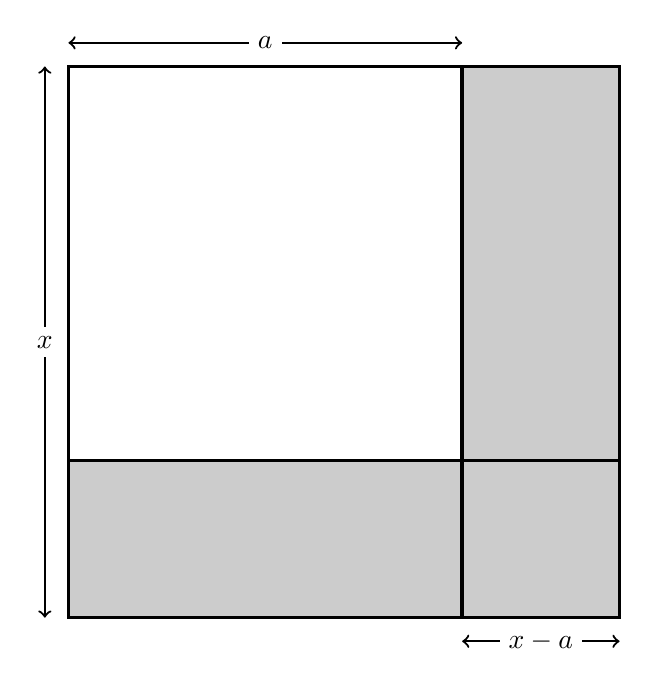
\begin{tikzpicture}[%%
  arrowStyle/.style={<->,thick},%%
  dashStyle/.style={-,dashed,very thick},%%
  labelStyle/.style={fill=white},%%
  lineStyle/.style={-,very thick},%%
  shadeStyle/.style={-,very thick,fill=gray!40}%%
]
%%
%%
\pgfmathsetmacro{\dx}{0.3} %% the gap between shape and label
\pgfmathsetmacro{\xlow}{0}
\pgfmathsetmacro{\xside}{7}
\pgfmathsetmacro{\ylow}{\xlow}
\pgfmathsetmacro{\dxa}{2}  %% the gap between x^2 and a^2
\pgfmathsetmacro{\da}{\xside-\dxa}  %% the side length a
%%
%% Coordinates for the larger square x^2.
\coordinate (xlowerLeft) at (\xlow,\ylow);
\coordinate (xupperRight) at (\xside,\xside);
%%
\normalsize
%%
%% Shade the required region.  This region is the difference of the
%% two squares.  Must shade first.
\draw[shadeStyle] (xlowerLeft) rectangle (\xside,\dxa);
\draw[shadeStyle] (\da,\dxa) rectangle (xupperRight);
%%
%% Draw and label the square for x^2.
%% Draw the square for x^2.
\draw[lineStyle] (xlowerLeft) rectangle (xupperRight);
%% Label the width of the square x^2.
\draw[arrowStyle] (\xlow-\dx,\ylow) -- (\xlow-\dx,\xside);
\node[labelStyle] at (\xlow-\dx,\xside/2) {$x$};
%%
%% Draw and label the square for a^2.
%% Draw the square for a^2.
\draw[lineStyle] (\xlow,\dxa) -- (\xside,\dxa);
\draw[lineStyle] (\da,\ylow) -- (\da,\xside);
%% Label the width of the square a^2.
\draw[arrowStyle] (\xlow,\xside+\dx) -- (\da,\xside+\dx);
\node[labelStyle] at (\xside*0.5-\dxa*0.5,\xside+\dx) {$a$};
%%
%% Label the width of the shaded region.
\draw[arrowStyle] (\xside-\dxa,\ylow-\dx) -- (\xside,\ylow-\dx);
\node[labelStyle] at (\da+\xside*0.5-\da*0.5,\ylow-\dx) {$x - a$};
\end{tikzpicture}

\end{document}
